\documentclass{article}
\usepackage[margin=1in]{geometry}
\usepackage{amsmath,amsthm,amssymb}
\usepackage{bbm,enumerate,mathtools}
\usepackage{tikz,pgfplots}
\usepackage{chessboard}
\usepackage[hidelinks]{hyperref}
\usepackage{multicol} % Problem 35

\newenvironment{question}{\begin{trivlist}\item[\textbf{Question.}]}{\end{trivlist}}
\newenvironment{note}{\begin{trivlist}\item[\textbf{Note.}]}{\end{trivlist}}
\newenvironment{references}{\begin{trivlist}\item[\textbf{References.}]}{\end{trivlist}}
\newenvironment{related}{\begin{trivlist}\item[\textbf{Related.}]\end{trivlist}\begin{enumerate}}{\end{enumerate}}


\begin{document}
\rating{4}{2}
Consider walks in a city, starting mid-block, where (1) at each intersection
the walker goes left right or straight, (2) at each mid-block, the walker
decides whether or not to turn around, and (3) she ends up back at her
apartment.
\begin{figure}[!h]
  \centering
  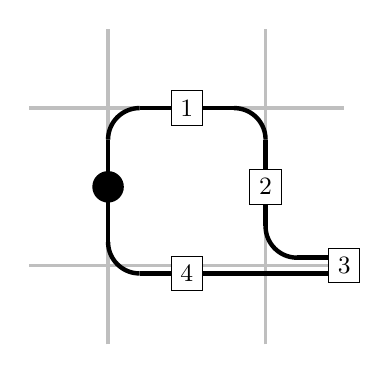
\begin{tikzpicture}[scale=2]
    \draw[very thick, gray!50] (-0.5, 0.5) grid (1.5, 2.5);
    \draw[ultra thick] (0,1.5)--(0,1.8);
    \draw[ultra thick, domain=90:180] plot ({cos(\x)/5 + 0.2}, {sin(\x)/5 + 1.8});
    \draw[ultra thick] (0.2,2)--(0.5,2);

    \draw[ultra thick] (0.5,2)--(0.8,2);
    \draw[ultra thick, domain=0:90] plot ({cos(\x)/5 + 0.8}, {sin(\x)/5 + 1.8});
    \draw[ultra thick] (1,1.8)--(1,1.5);

    \draw[ultra thick] (1,1.5)--(1,1.25);
    \draw[ultra thick, domain=180:270] plot ({cos(\x)/5 + 1.2}, {sin(\x)/5 + 1.25});
    \draw[ultra thick] (1.2,1.05)--(1.5,1.05);

    \draw[ultra thick] (1.5,0.95)--(0.5,0.95);

    \draw[ultra thick] (0.5,0.95)--(0.2,0.95);
    \draw[ultra thick, domain=180:270] plot ({cos(\x)/5 + 0.2}, {sin(\x)/5 + 1.15});
    \draw[ultra thick] (0,1.15)--(0,1.5);

    \node[draw={},fill=white] at (0.5,2) {\small 1};
    \node[draw={},fill=white] at (1,1.5) {\small 2};
    \node[draw={},fill=white] at (1.5,1) {\small 3};
    \node[draw={},fill=white] at (0.5,0.95) {\small 4};
    \fill (0,1.5) circle (0.1cm);


  \end{tikzpicture}
  \caption{
    An example of a 5-step walk returning to the apartment.
  }
\end{figure}
\begin{question}
  How many $n$-block walks can the walker take?
\end{question}
\begin{related}
  \item What if the walker does not want to walk along the same strip of road
    twice?
  \item What if the walker does not want to walk along the same \textit{side} of
    the same strip of road? (Suppose she always walks on the right side of the
    street.)
  \item What if the walker never wants to revisit the same intersection?
  \item How many walks up to dihedral action?
  \item What if the walker does not turn around?
  \item What if the walker never goes straight? Never goes right?
\end{related}
\begin{references}
  \item Problem 46.
\end{references}

\end{document}
